\documentclass[12pt]{article}
\usepackage{parskip}
\usepackage[letterpaper, margin=1in]{geometry}
\usepackage{graphicx}
\usepackage{amsmath}
\usepackage{enumitem}
\usepackage{caption}
\usepackage{subcaption}
\usepackage{hyperref}
\graphicspath{{./images/}}
\title{ELECENG 3EJ4 Lab 4}
\author{Raeed Hassan \\ hassam41 \\ McMaster University}
\begin{document}
\maketitle
\clearpage
\begin{itemize}
    \section*{Part 1}
    \item [\textbf{Q1.}]
    \begin{enumerate}
        \item Based on the simulation data obtained in Step 1.2, the low-frequency voltage gains in dB are: $A_{d1} = 7.38$, $A_{d2} = 70.05$, and $A_{d3} = 0$.
        \item Based on the simulation data obtained in Step 1.2, the overall voltage gain for the differential-mode signal is $A_d = 77.43$ dB or $A_d = 7437.8$ (real magnitude).
        \item The non-inverting input of the operational amplifier is $V_2$, as the simulated phase of the output voltage $V_o$ is in phase with the phase offset of $V_2$ at low-frequency.
        \item The upper 3-dB frequency $f_H$ of the operational amplifier is approximately 6.4 kHz, and this value was determined the frequency when the phase drops by 45 degrees from its initial value.
    \end{enumerate}
    \item [\textbf{Q2.}]
    The differential-mode gain $A_{d1}$ in Q1, 7.38 dB, is around one-tenth of the differential-mode gain $A_{d}$ in Lab 3, 70.07 dB. The difference is due to the feedback received by the emitters of the PNPs in the current mirror, affecting the collector current at the output of the differential amplifier (likely an increase in emitter currents causing a decrease in voltage gain).
    \item [\textbf{Q3.}]
    Based on the simulated results obtained in Step 1.2 and 1.3, the input resistance $R_{in} = 81.757$ k$\Omega$ and the output resistance $R_o = 461$ $\Omega$. This matches the expected resistances for an operational amplifier, a high input resistance and a low output resistance.
    \begin{figure}[!ht]
        \centering
        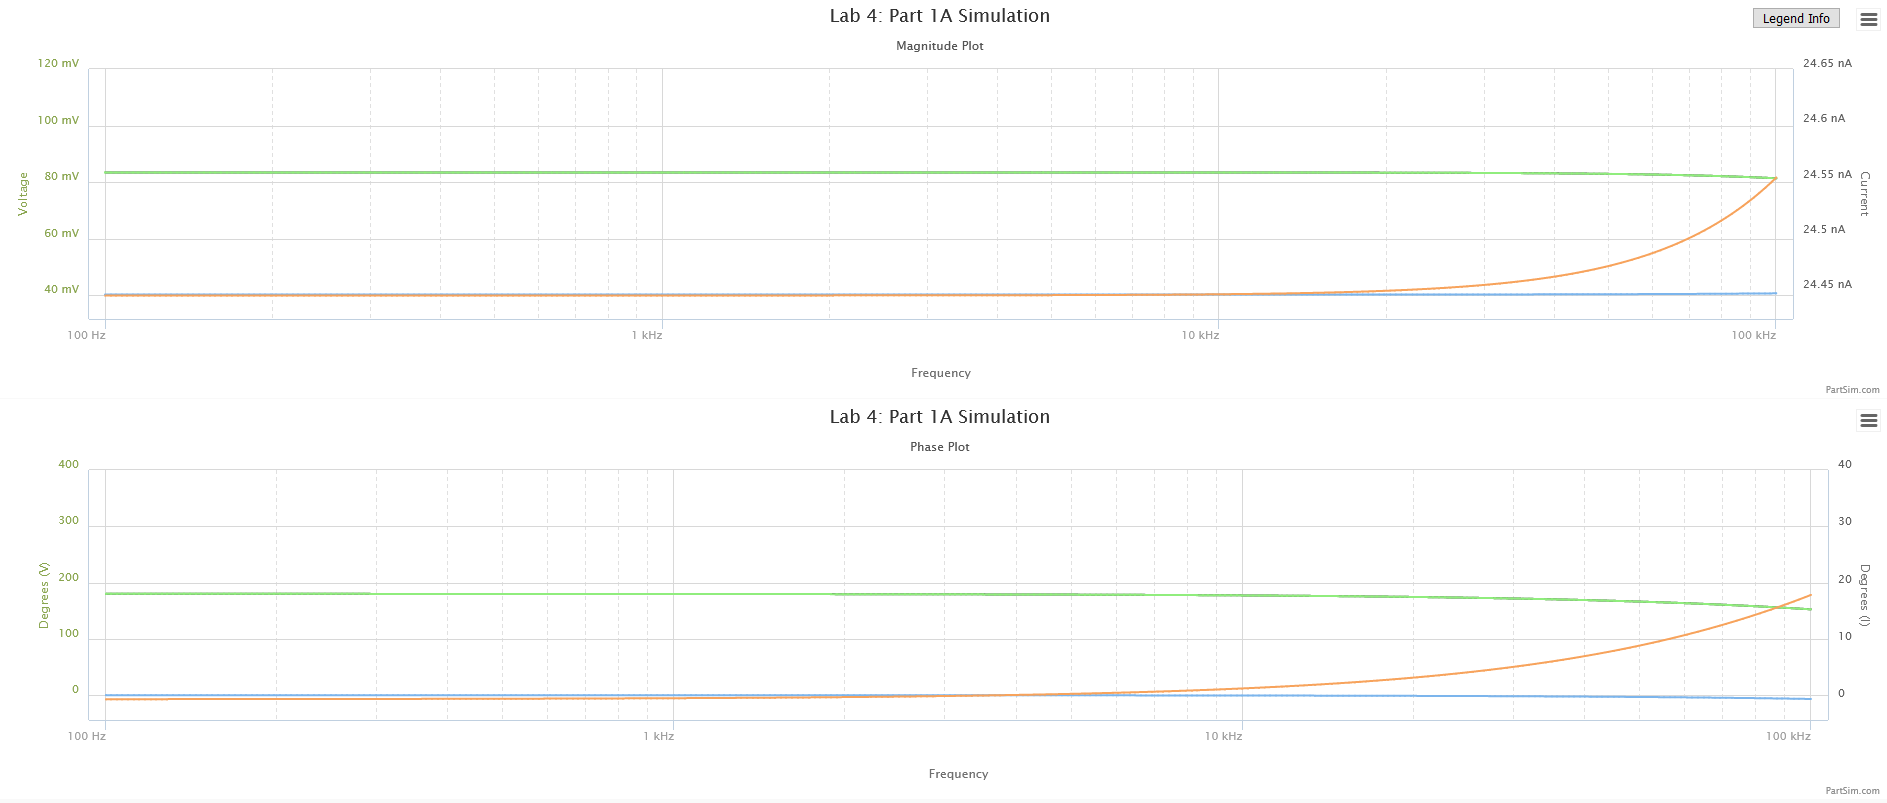
\includegraphics[width=\textwidth]{Step1.2}
        \caption{\label{Step1.2}Bode plots for Step 1.2 (Green/Black: $V_o$/$V_{o2}$, Orange: $i_{b1}$, Blue: $V_{o1}$)}
    \end{figure}
    \begin{figure}[!ht]
        \centering
        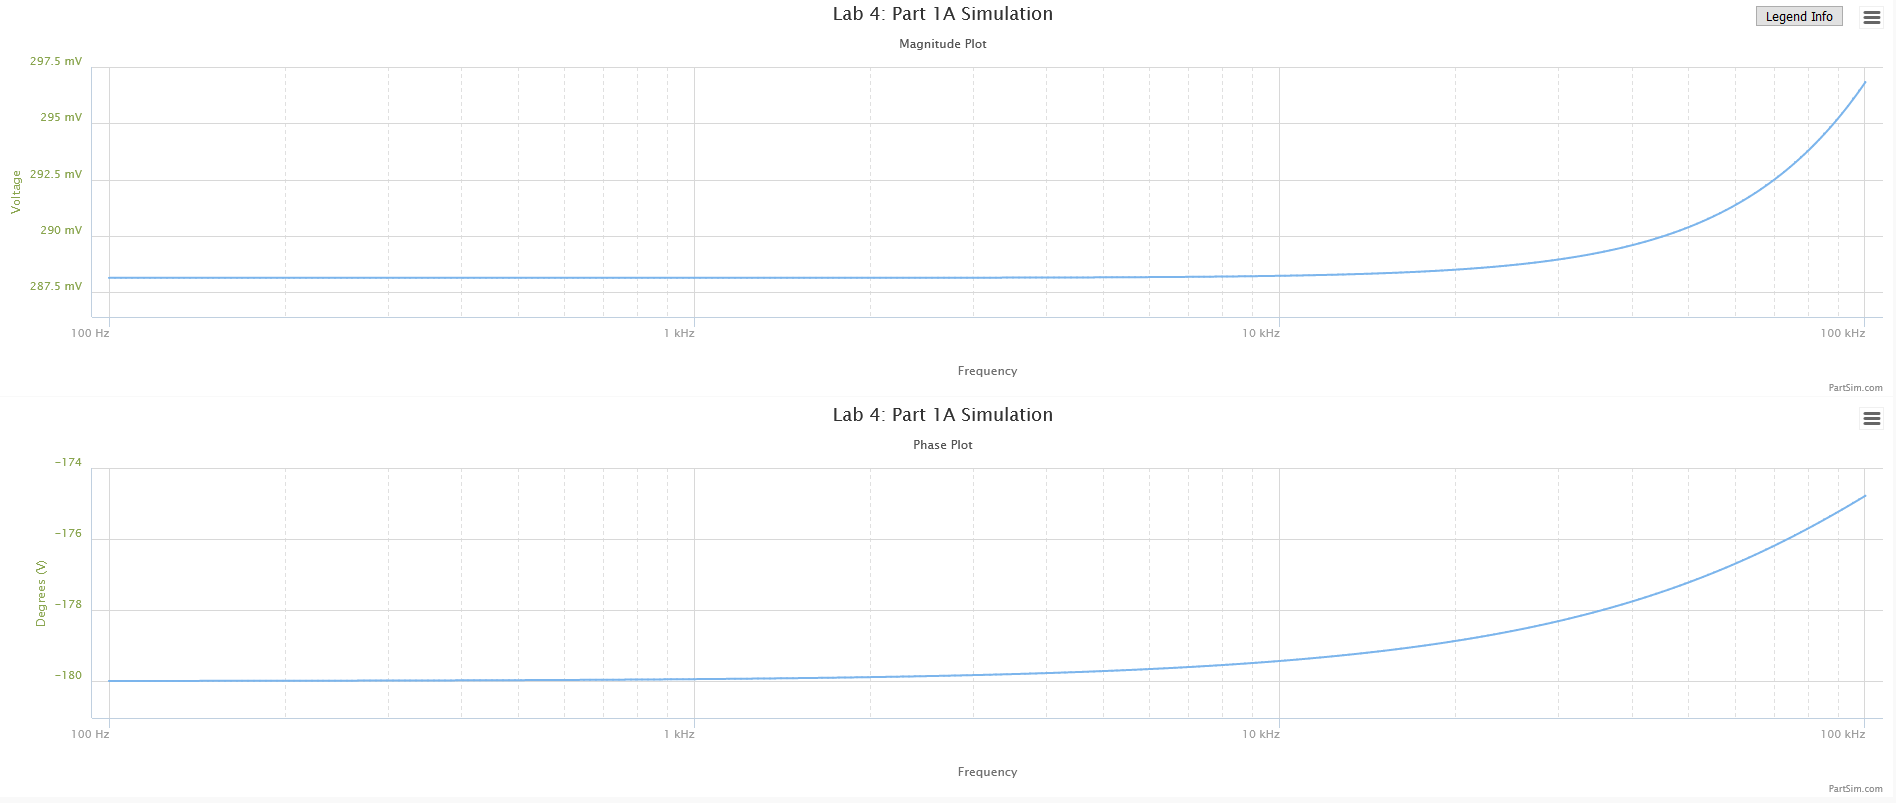
\includegraphics[width=\textwidth]{Step1.3}
        \caption{\label{Step1.3}Bode plots for Step 1.3}
    \end{figure} \newpage
    \item [\textbf{Q4.}]
    \begin{enumerate}
        \item The plots for the simulated and measured results from Steps 1.6 and 1.11 for the output voltage $V_o$ vs. the time characteristics at 1 KHz are shown in Figure \ref{fig:Q4}.
        \begin{figure}[!ht]
            \centering
            \begin{subfigure}{0.49\textwidth}
                \centering
                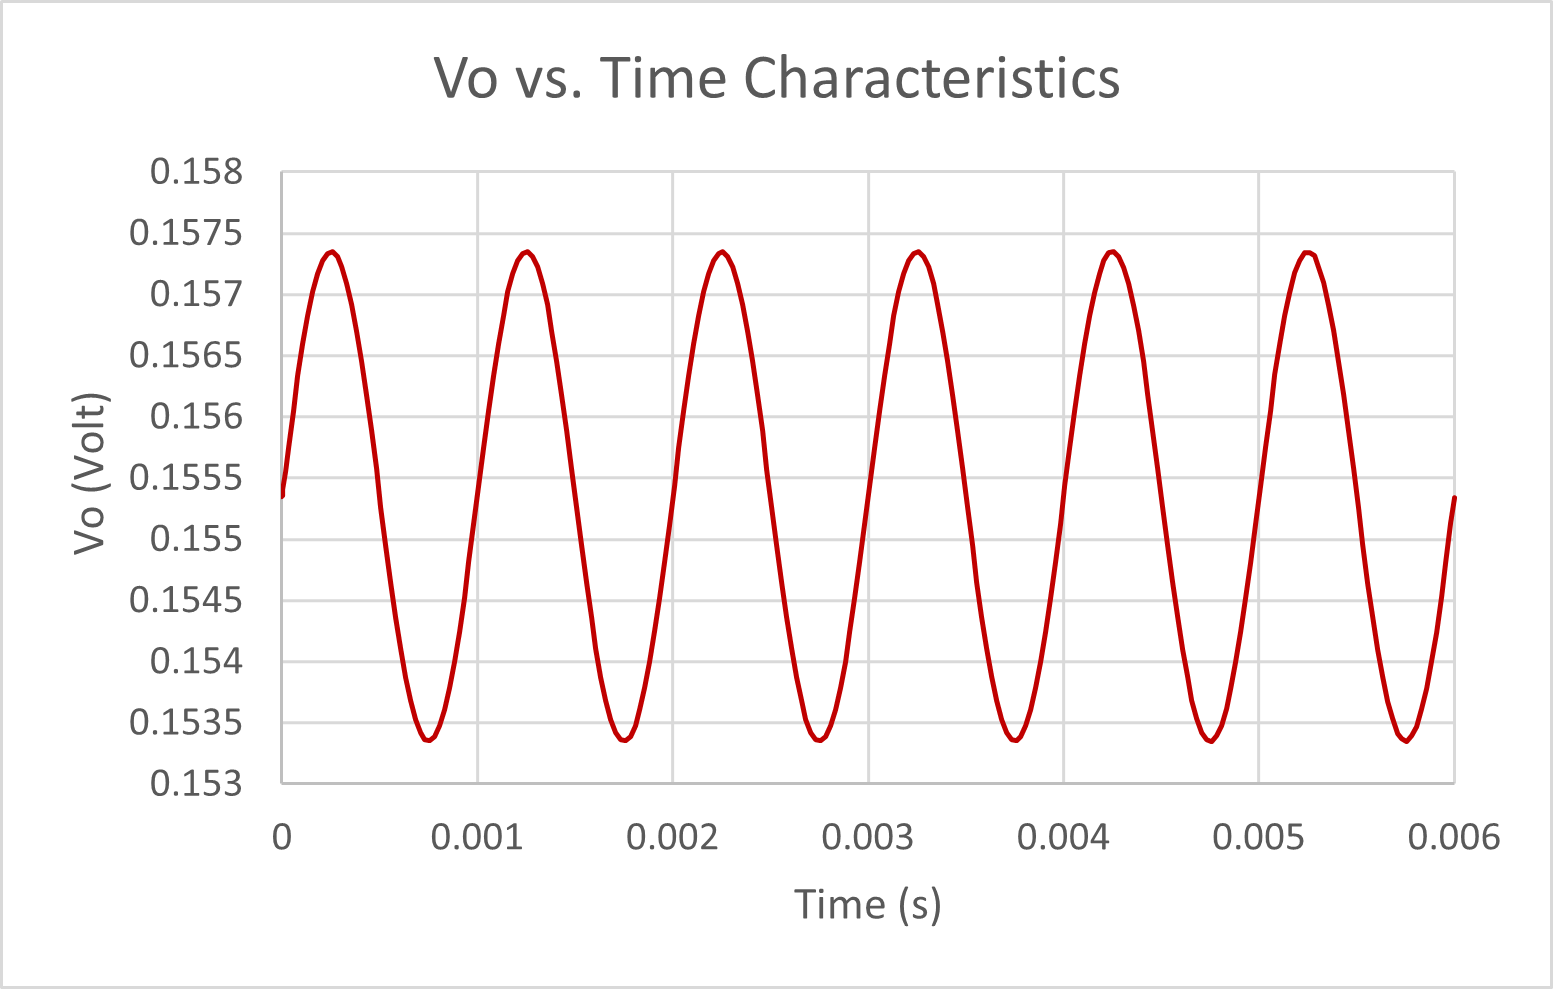
\includegraphics[width=\textwidth]{Q4Sim}
                \caption{\label{fig:Q4Sim}Step 1.6 (Simulated) Plot}
            \end{subfigure}
            \begin{subfigure}{0.49\textwidth}
                \centering
                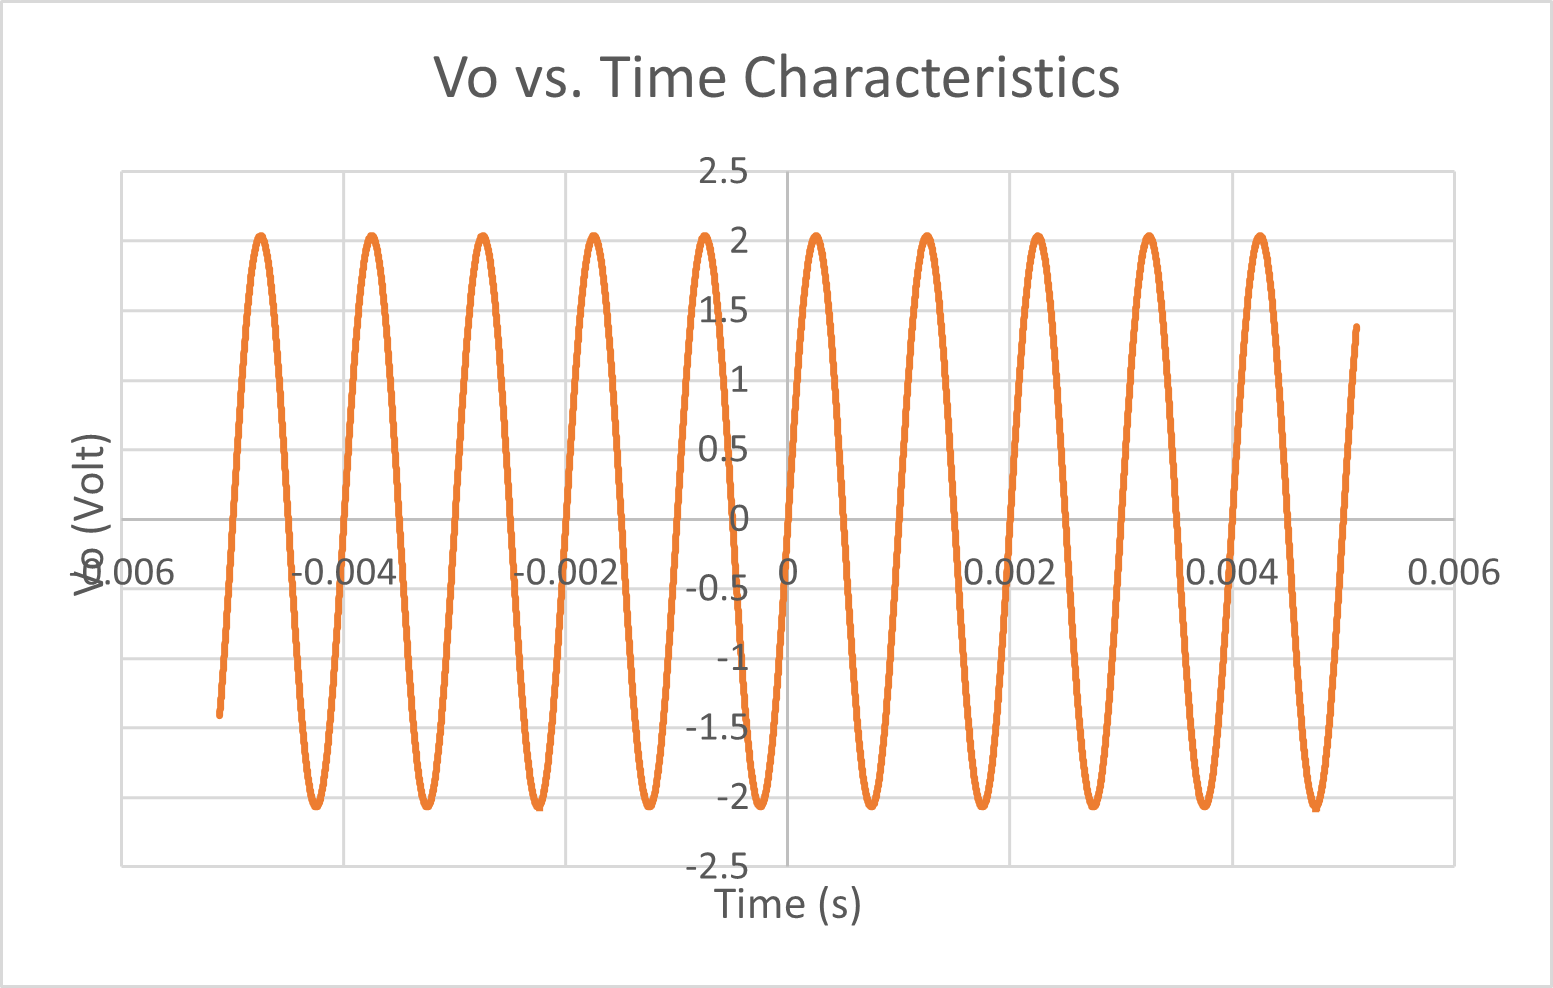
\includegraphics[width=\textwidth]{Q4Measure}
                \caption{\label{fig:Q4Measure}Step 1.11 (Measured) Plot}
            \end{subfigure}
            \caption{\label{fig:Q4}Output voltage $V_o$ vs. time characteristics at 1 kHz}
        \end{figure}
        \item The peak to peak voltage, $V_{pp}$ for the simulated results is 40 mV, while the peak to peak voltage, $V_{pp}$, for the measured results is around 4 V. The AC amplitude, $V_p$ and DC voltages, $V_{dc}$ for the simulated results are 20 mV and 155 mV, while $V_p$ and $V_{dc}$ for the measured results are 2 V and -15 mV. The differences in $V_{pp}$ and $V_p$ voltages are explained by the different input AC voltages at $V_1$, the input for the measurement is 1000 times greater than the input for the simulation, therefore the measured peak to peak voltage and AC voltage are 1000 times greater than the simulated peak to peak voltage and AC voltage. Otherwise, both sets of data have the same frequency/period and exhibit the same behaviour.
    \end{enumerate}
    \item [\textbf{Q5.}]
    \begin{enumerate}
        \item The plots for the simulated and measured results from Steps 1.7 and 1.12 for the voltage gain magnitude and phase vs. frequency characteristics are shown in Figure \ref{fig:Q5}.
        \begin{figure}[!ht]
            \centering
            \begin{subfigure}{0.49\textwidth}
                \centering
                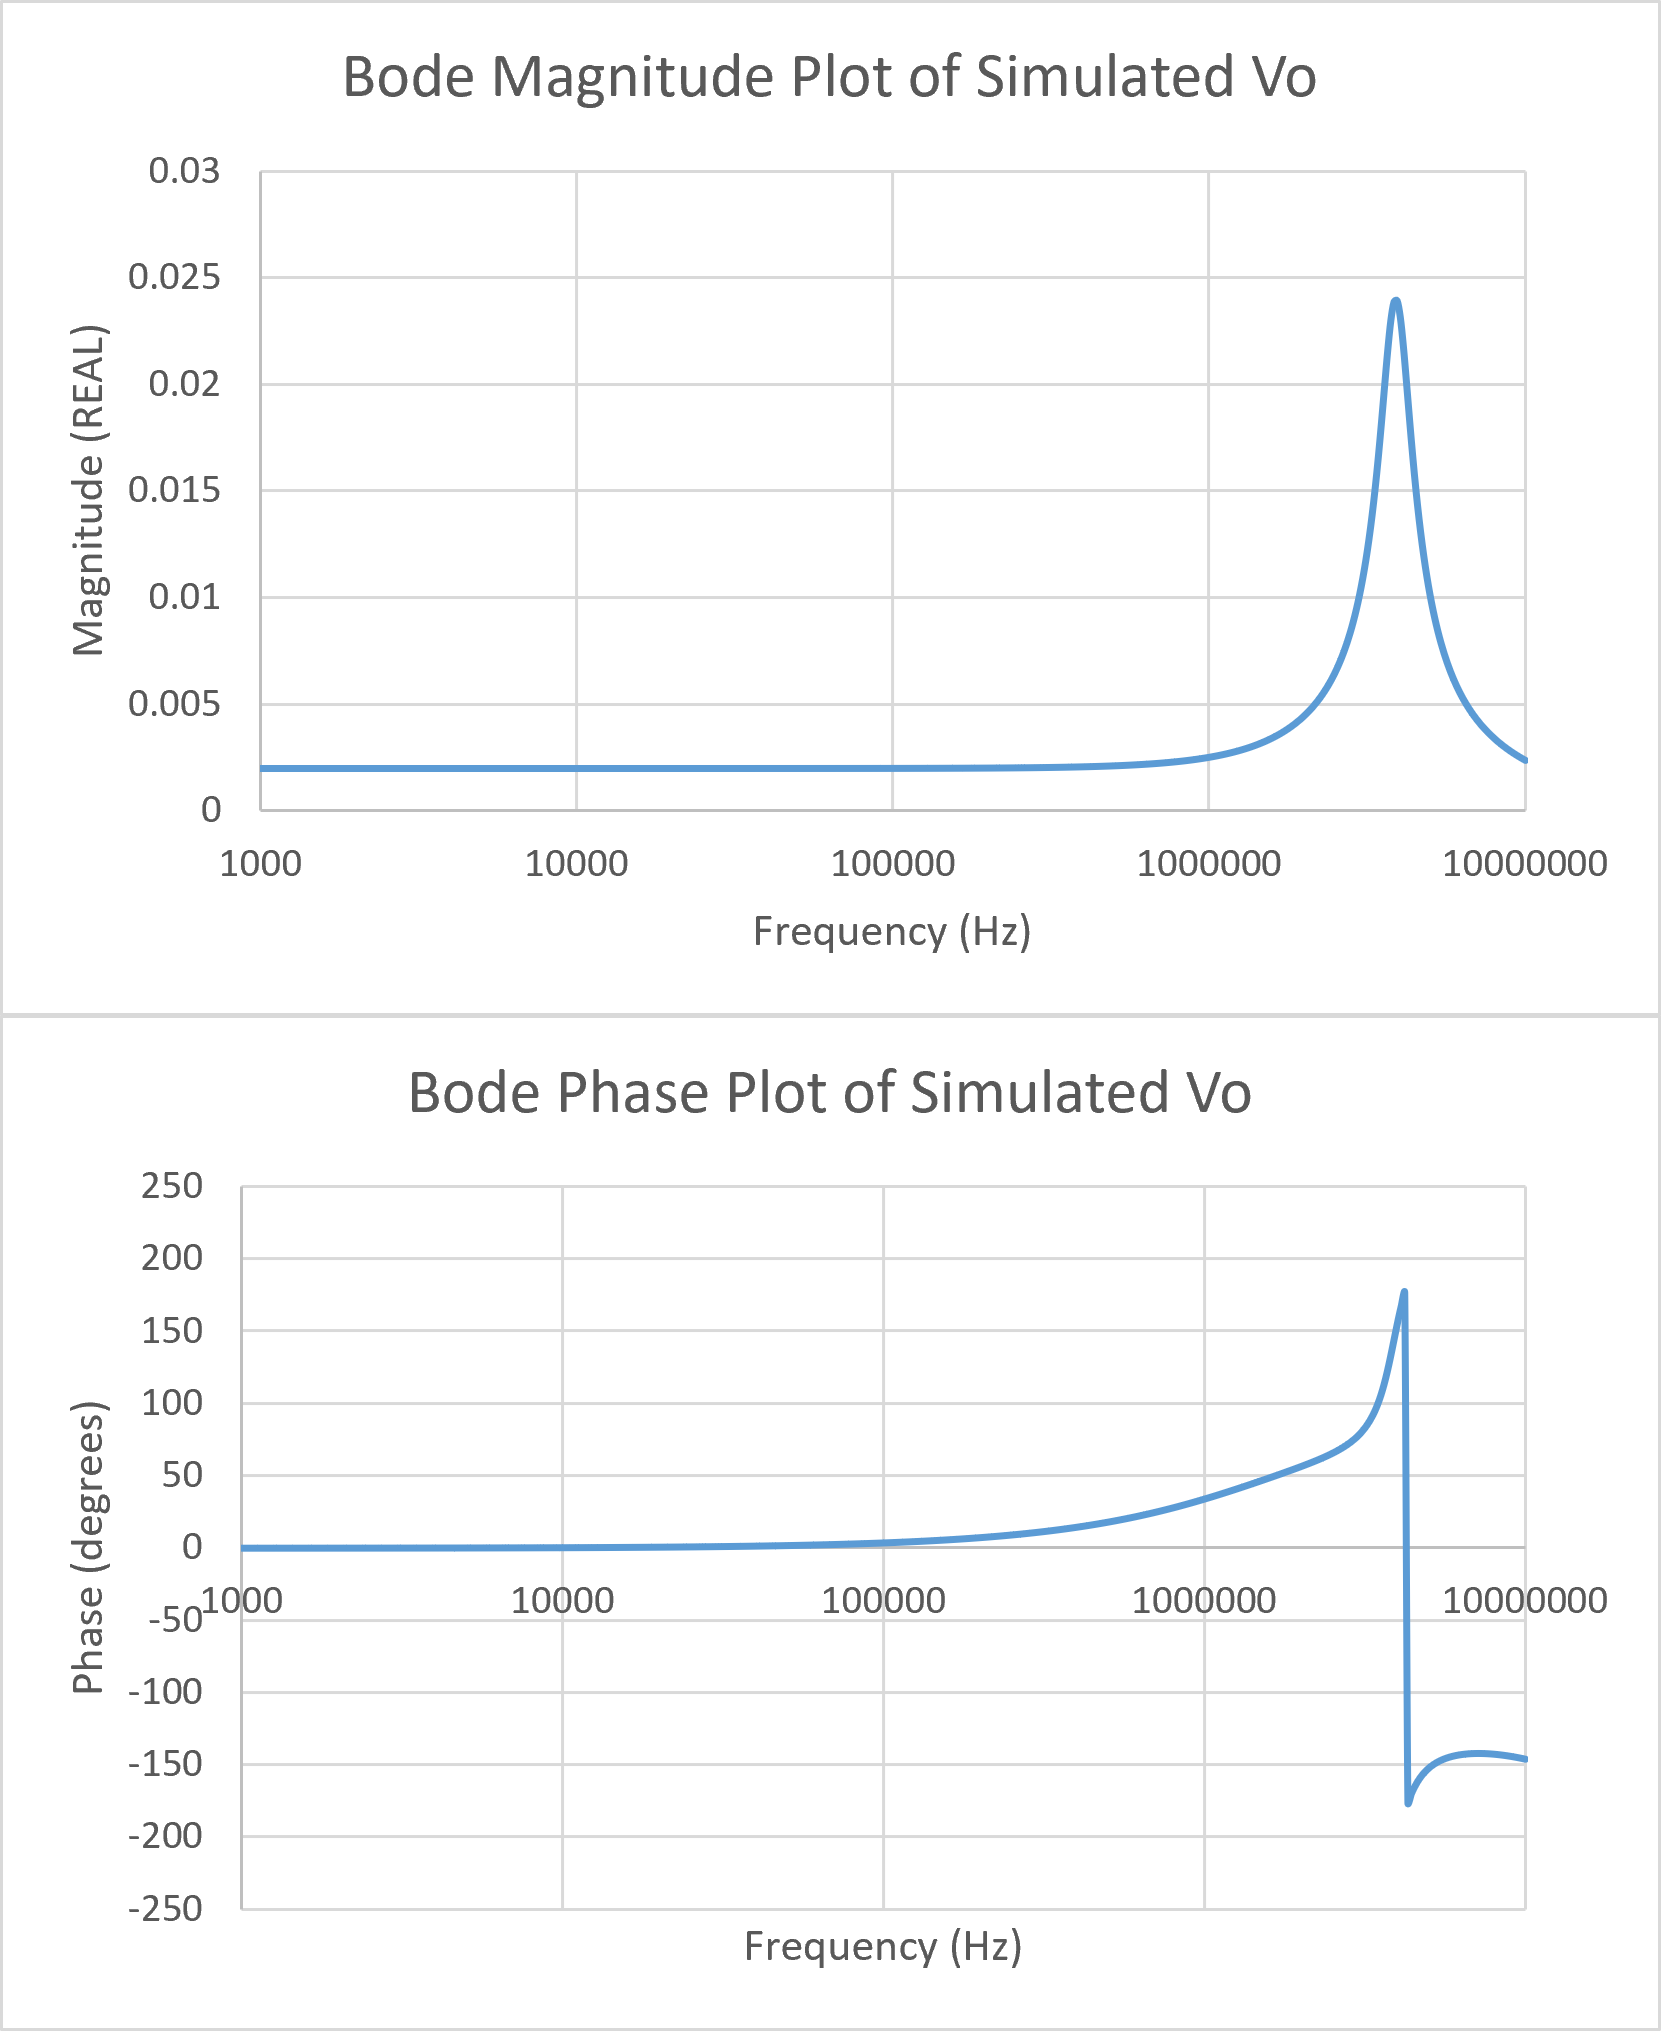
\includegraphics[width=\textwidth]{Q5Sim}
                \caption{\label{fig:Q5Sim}Step 1.7 (Simulated) Plot}
            \end{subfigure}
            \begin{subfigure}{0.49\textwidth}
                \centering
                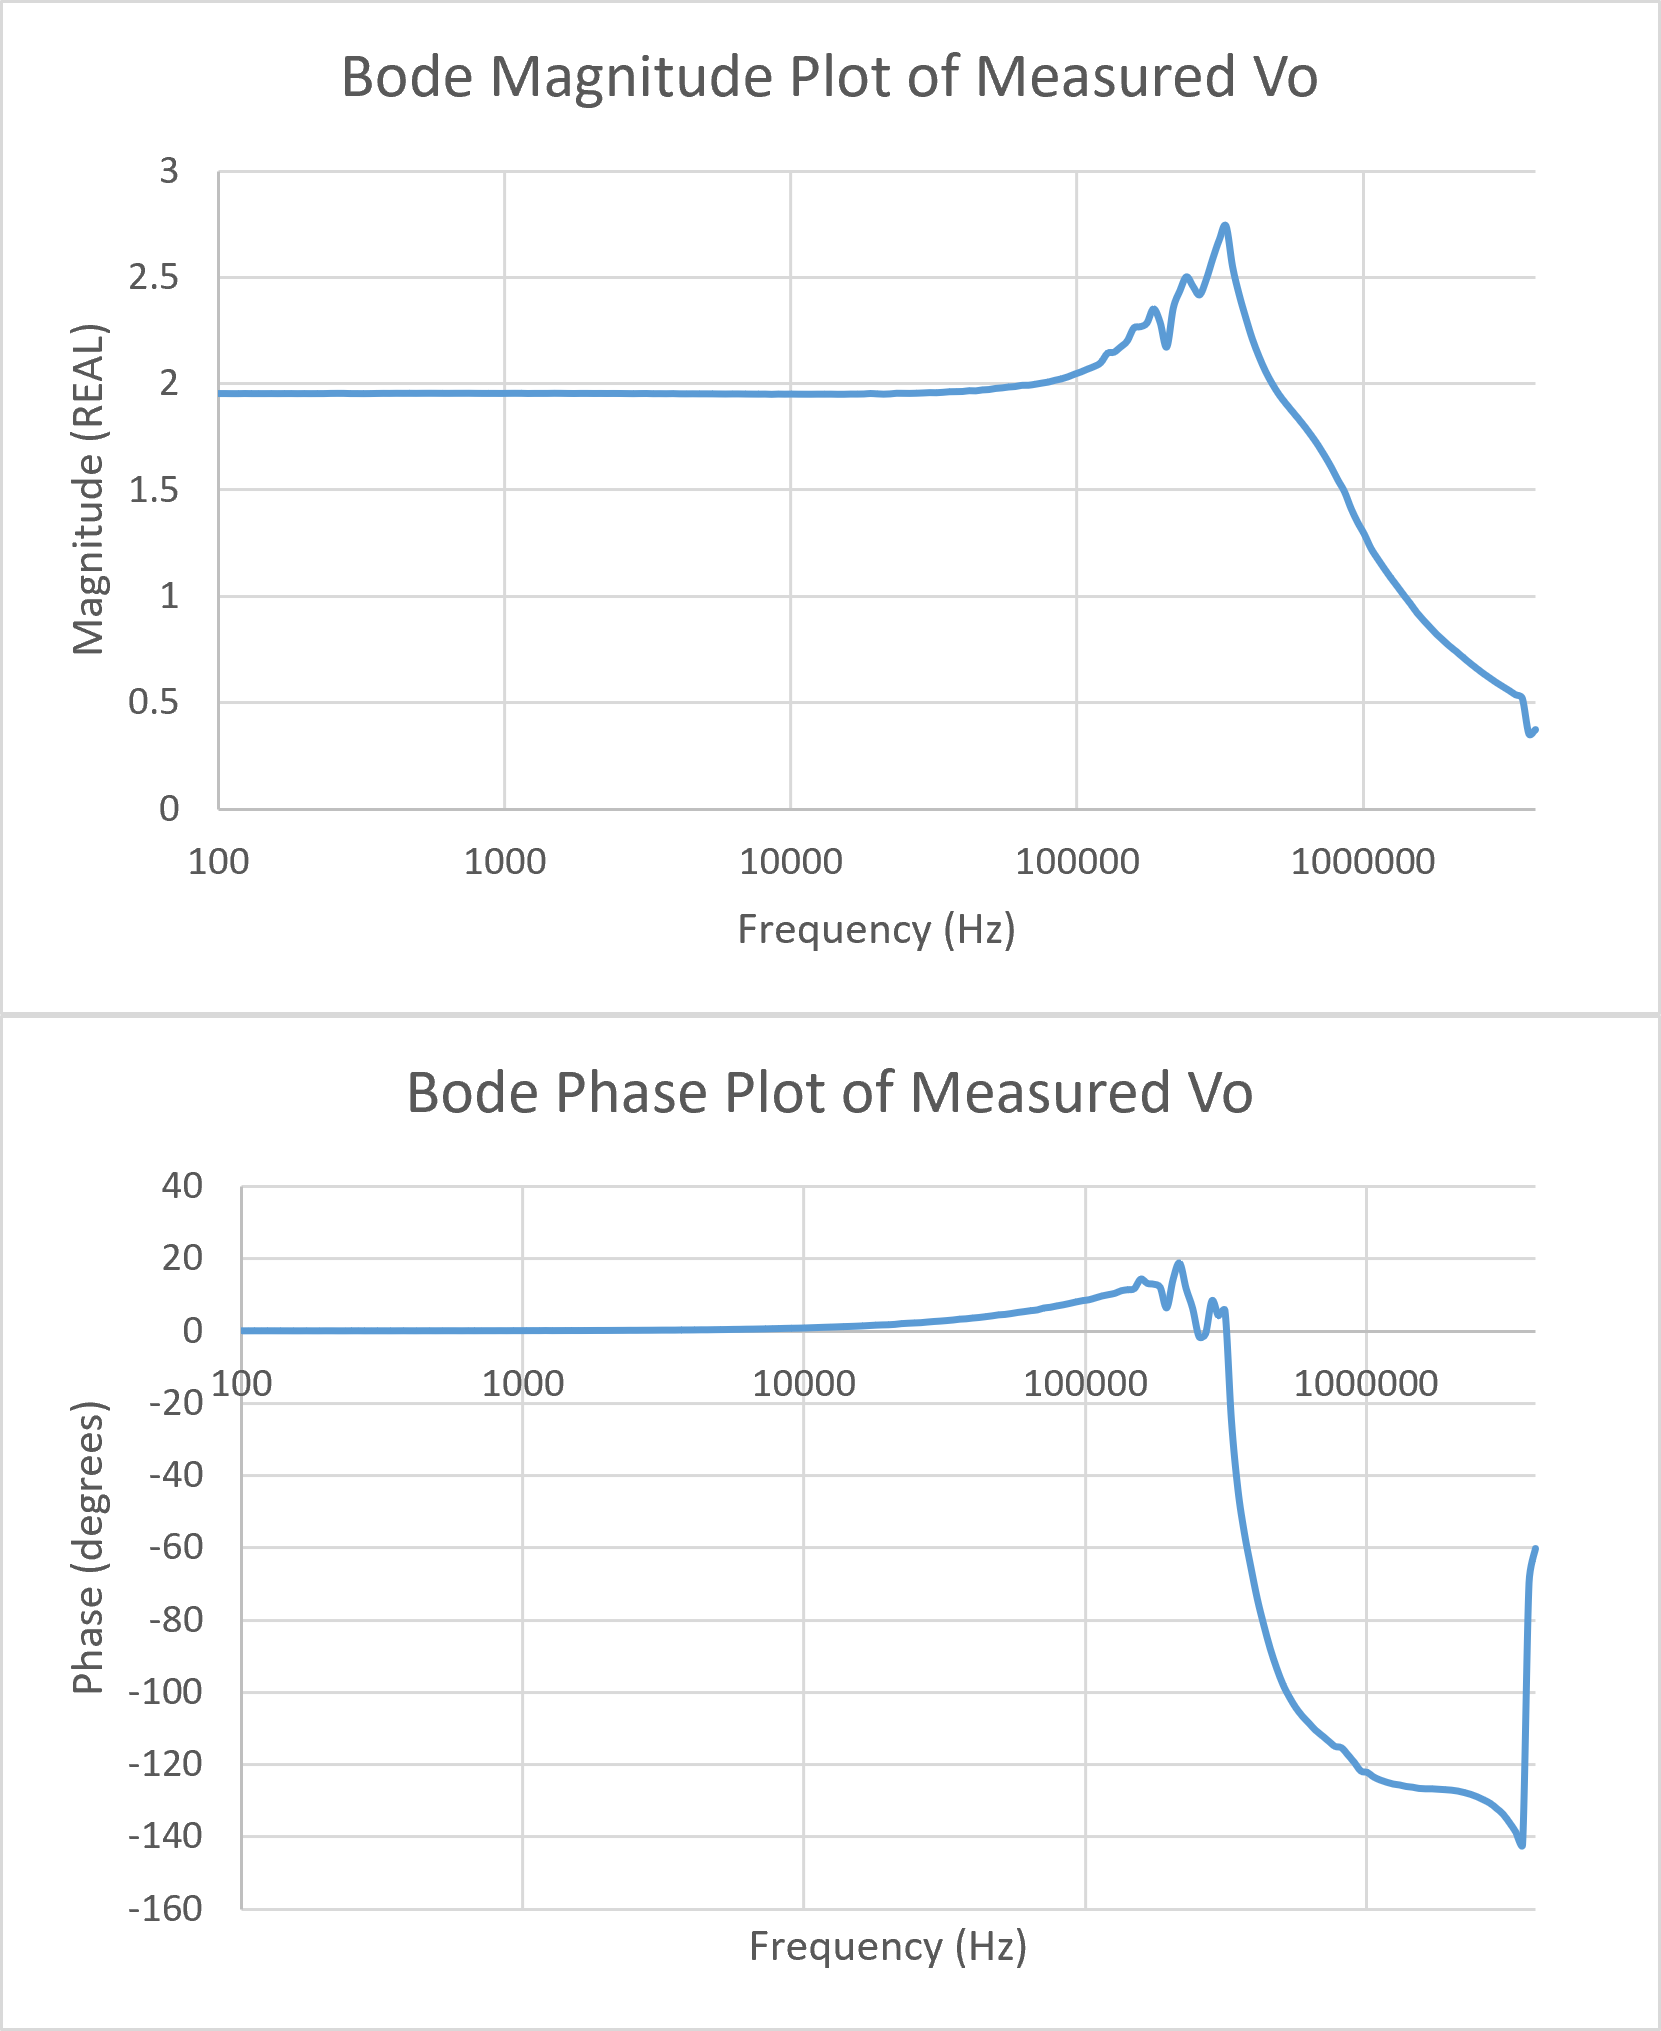
\includegraphics[width=\textwidth]{Q5Measure}
                \caption{\label{fig:Q5Measure}Step 1.12 (Measured) Plot}
            \end{subfigure}
            \caption{\label{fig:Q5}Bode plots for Step 1.7 and 1.12}
        \end{figure}
        \item Similar to Q4, the bode magnitude plots display similar behaviour (albeit at much lower frequencies), but have different very different scales due to the 1 mV input AC voltage in simulation, causing the magnitude gain to be 1000 times smaller in the simulated results. If the simulation is done with the same input AC voltage (1 V), the resulting bode magnitude plot has the same behaviour as before, but matches the scale of the magnitude gain seen in the measured bode magnitude plot. The bode phase plot also displays the same general behaviour, beginning to increase at a certain frequency before having a steep drop in the phase. The behaviour towards the end of the plot begins to slightly differ. This due to a number of factors such as the internal capacitances in all of the BJTs affecting the phase at higher frequencies, or other components of the physical circuit behaving differently than expected in simulation at higher frequencies (breadboard, wires, AD2 board) despite behaving the same at lower frequencies.
    \end{enumerate}
    \item [\textbf{Q6.}]
    The circuit uses a series-shunt feedback configuration. The input is connected directly into the directional amplifier, resulting in a series connection, while the output provides a feedback to the differential amplifier, resulting in a shunt connection.
    \item [\textbf{Q7.}]
    The beta network consists of $R_1$ and $R_2$, and the value of $\beta$ is $\frac{R_1}{R_1+R_2} = 0.5$. The feedback components $R_{11}$ and $R_{22}$ are simply $R_{11} = R_1 = 100$ k$\Omega$ and $R_{22} = R_2 = 100$ k$\Omega$. 
    \item [\textbf{Q8.}]
    The series-shunt amplifier can be represented as a two port network with $h$ parameters. The voltage gain is equal to $\frac{1}{h_{12}}$ where $h_{12} = \beta$. Therefore the voltage gain, $A_v$, is $\frac{1}{0.5} = 2$. This voltage gain matches with the voltage gain, $A_v$, of 2 (or 6 dB) determined in the simulation done in Step 1.7. The input impedance $R_{in}$ is equal to $h_{11} = R_1 \parallel R_2 = 50$ k$\Omega$, and the output impedance $R_{o}$ is equal to $\frac{1}{h_{22}} = R_1 + R_2 = 200$ k$\Omega$.

    \clearpage
    \section*{Part 2}
    \item [\textbf{Q9.}]
    $C = C_1 = C_2$ and $R = R_3 = R_4$
    \begin{equation*}
    \begin{aligned}
        V_o &= V_+\left(1+\frac{1}{sCR}\right) + RV_+\left[\frac{1}{R} + sC\left(1 + \frac{1}{sCR}\right)\right] \\
        &= V_+\left(1+\frac{1}{sCR}\right) + V_+\left(2 + sCR\right) \\
        &= V_+(3 + \frac{1}{sCR} + sCR) \\
        \Rightarrow \frac{V_+}{V_o} &= \frac{s/CR}{s^2 + s(\frac{3}{CR}) + \left(\frac{1}{CR}\right)^2} \\
        L(s) &= \left(1+\frac{R2}{R1}\right)\frac{s/CR}{s^2 + s\frac{3}{CR} + \left(\frac{1}{CR}\right)^2}
    \end{aligned}
    \end{equation*}
    The zero loop phase frequency $\omega_0$ is $\omega_0 = \frac{1}{CR}$. At the zero loop phase frequency, $\lvert L(j\omega) \rvert = \frac{1}{3}\left(1+\frac{R2}{R1}\right)$, therefore for oscillation we require $\frac{1}{3}\left(1+\frac{R2}{R1}\right) \geq 1$ which occurs when $\frac{R2}{R1} \geq 2$.
    \item [\textbf{Q10.}]
    The characteristic equation of the system is $ 1 - L(s) = 1 - \left(1+\frac{R2}{R1}\right)\frac{s/CR}{s^2 + s\frac{3}{CR} + \left(\frac{1}{CR}\right)^2} = 0$. To find the pole $Q$, we can convert $L(s)$ into the frequency domain, can find that $L(j\omega) = \frac{j\omega\left[\frac{1+R_2/R_1}{CR}\right]}{\left[\left(\frac{1}{CR}\right)^2 - \omega^2\right] + j\frac{3\omega}{CR}}$. From this equation, we see that the value of $R_2/R_1 = 2$ will give us $j\frac{3\omega}{RC}$ in both the numerator and denominator, leaving us with $-\omega^2 - (\frac{1}{CR})^2$ or a pole Q at $(\frac{1}{CR})^2$ due to the Barkhausen Criterion.
    \item [\textbf{Q11.}]
    The settling times for R2 = 220 k$\Omega$, 240 k$\Omega$ and 280 k$\Omega$ are approximately 3.75 ms, 1.25 ms and 0.6 ms. The settling time decreases as the value of R2 increases. This behaviour is due to the loop gain $L(s)$ (derived in Q9) increasing as the value of R2 increases, decreasing the amount of time the oscillator circuit requires to reach saturation ($\lvert5\text{ V}\rvert$ for this circuit).
    \item [\textbf{Q12.}]
    \begin{enumerate}
        \item The plots for $V_o$ found in Steps 2.4, 2.6, 2.9, and 2.10 are shown in Figure \ref{fig:Q12}. The plots for 2.9 and 2.10 continue from after the oscillations have settled, but show the same behaviour as the simulated plots after settling, including sharing the same frequencies.
        \begin{figure}[!ht]
            \centering
            \begin{subfigure}{0.49\textwidth}
                \centering
                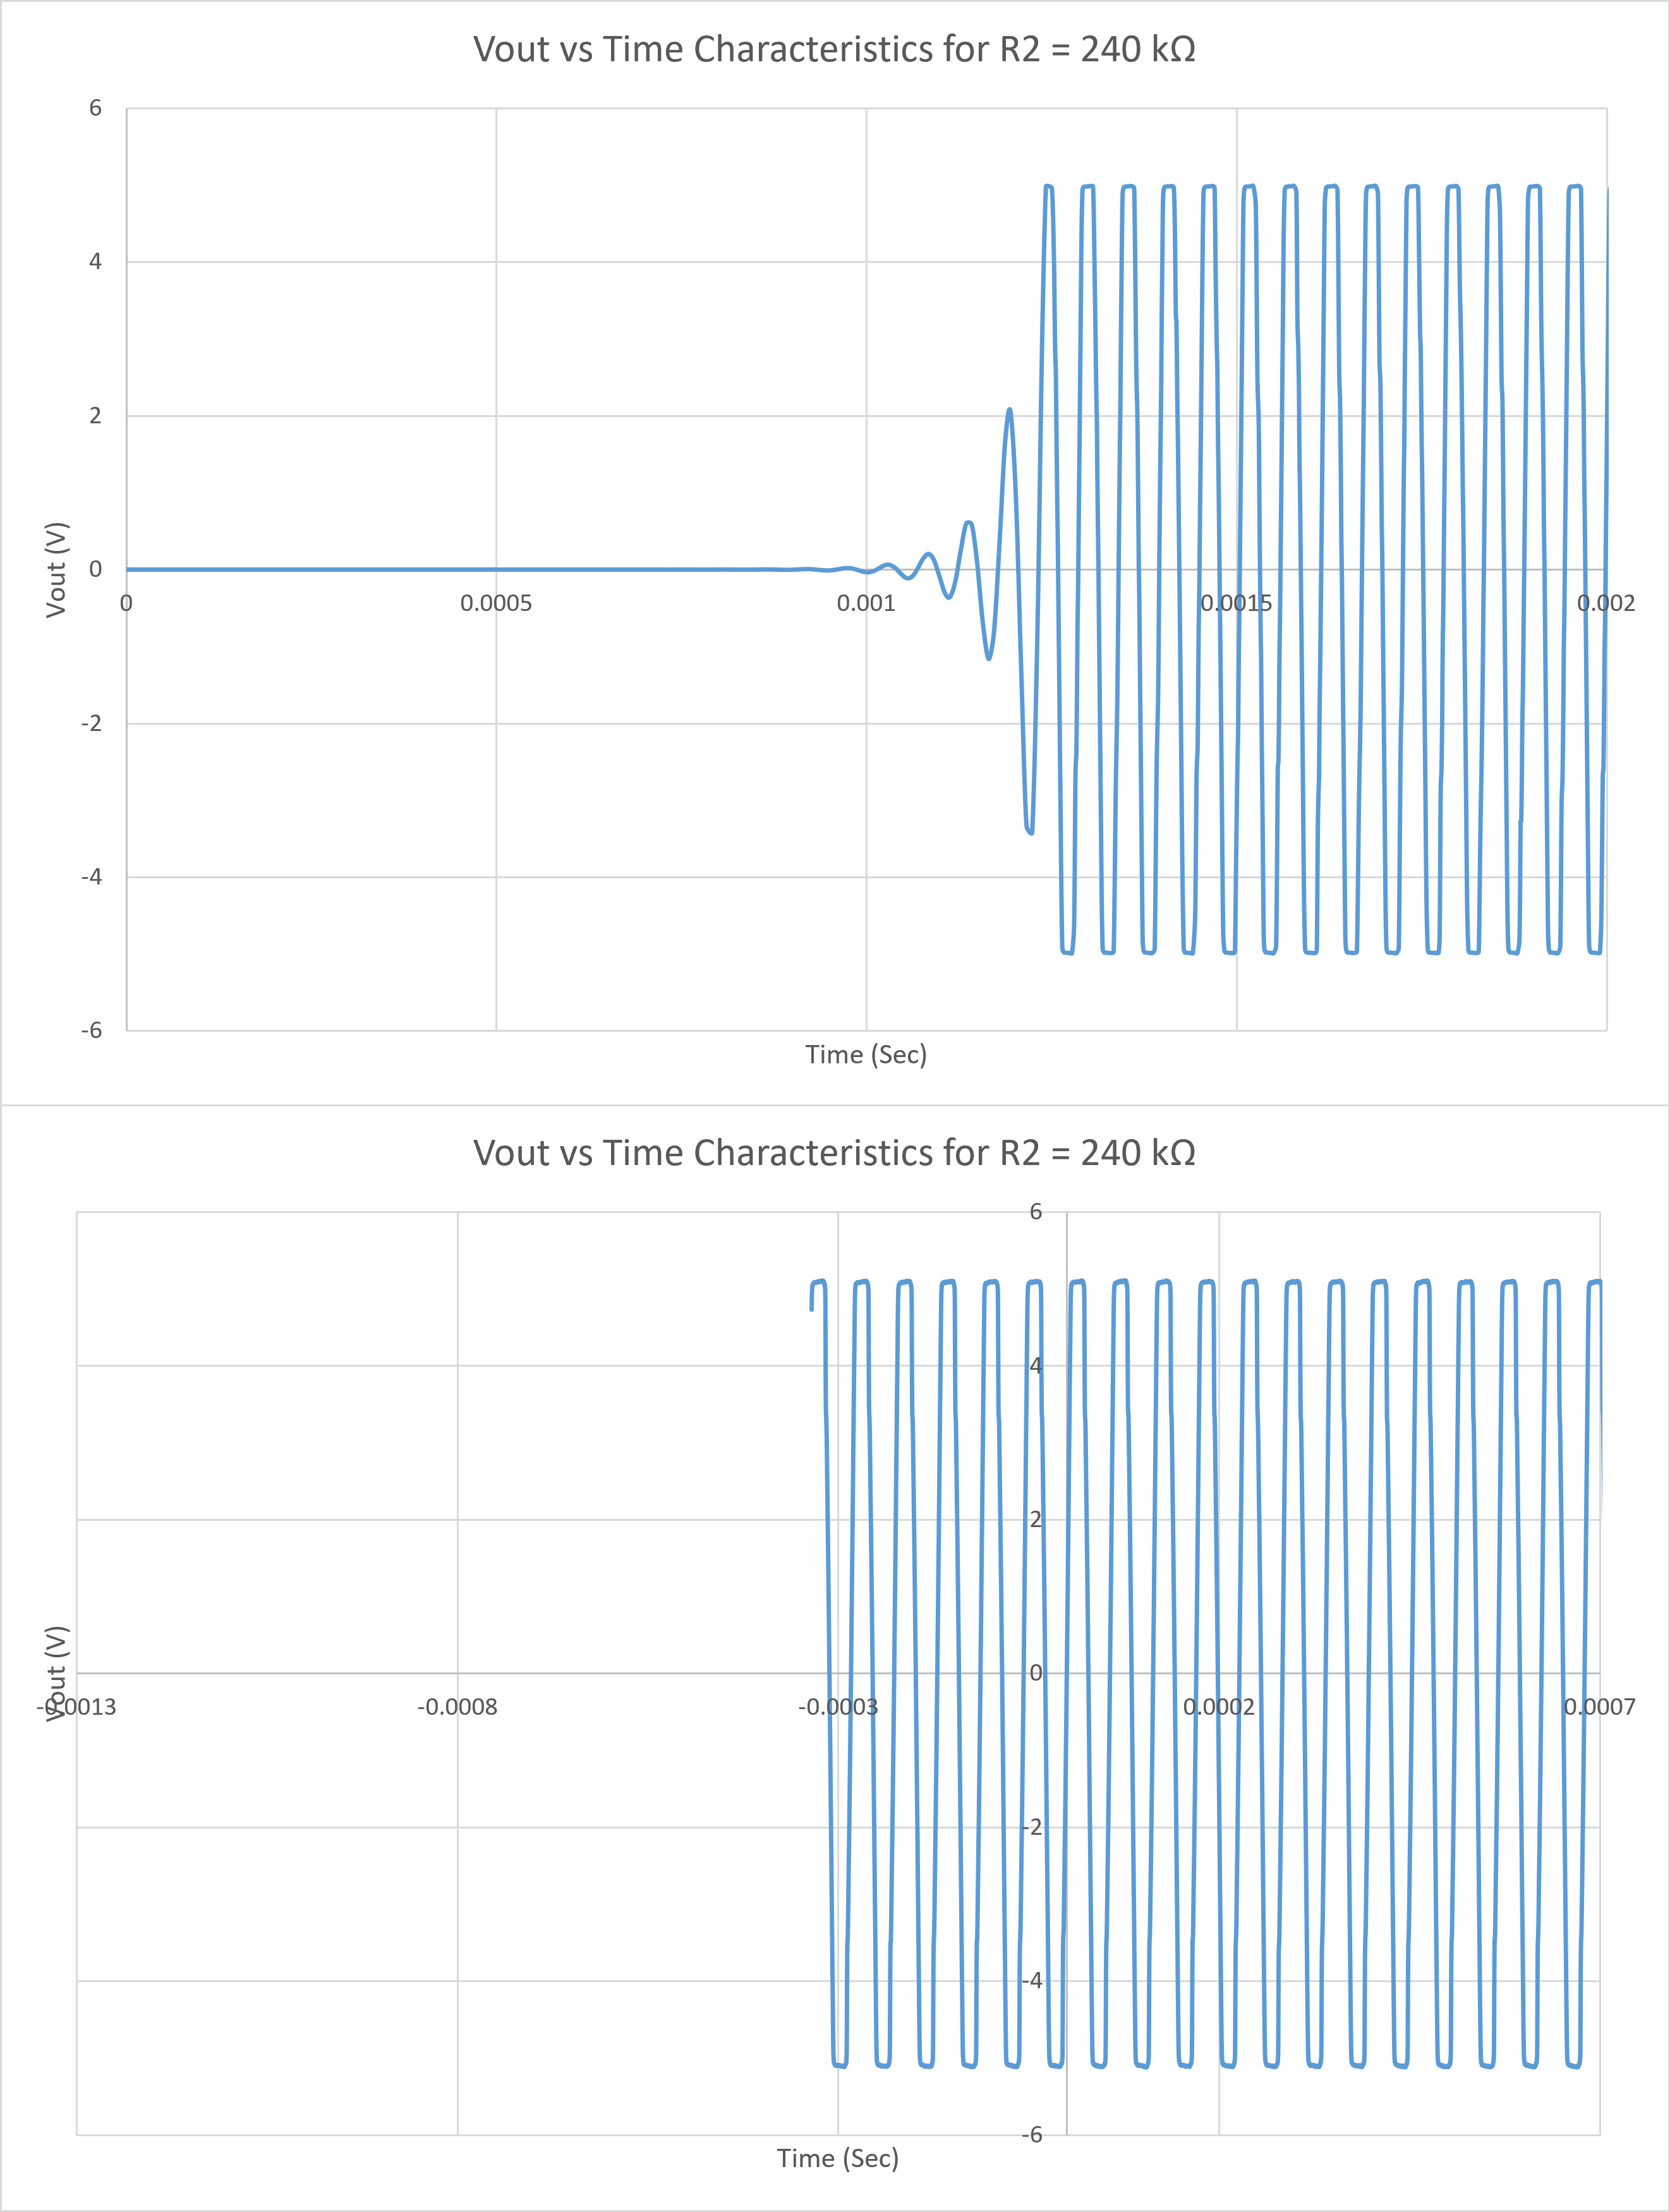
\includegraphics[width=\textwidth]{Q12A}
                \caption{\label{fig:Q12A}Steps 2.4 and 2.9}
            \end{subfigure}
            \begin{subfigure}{0.49\textwidth}
                \centering
                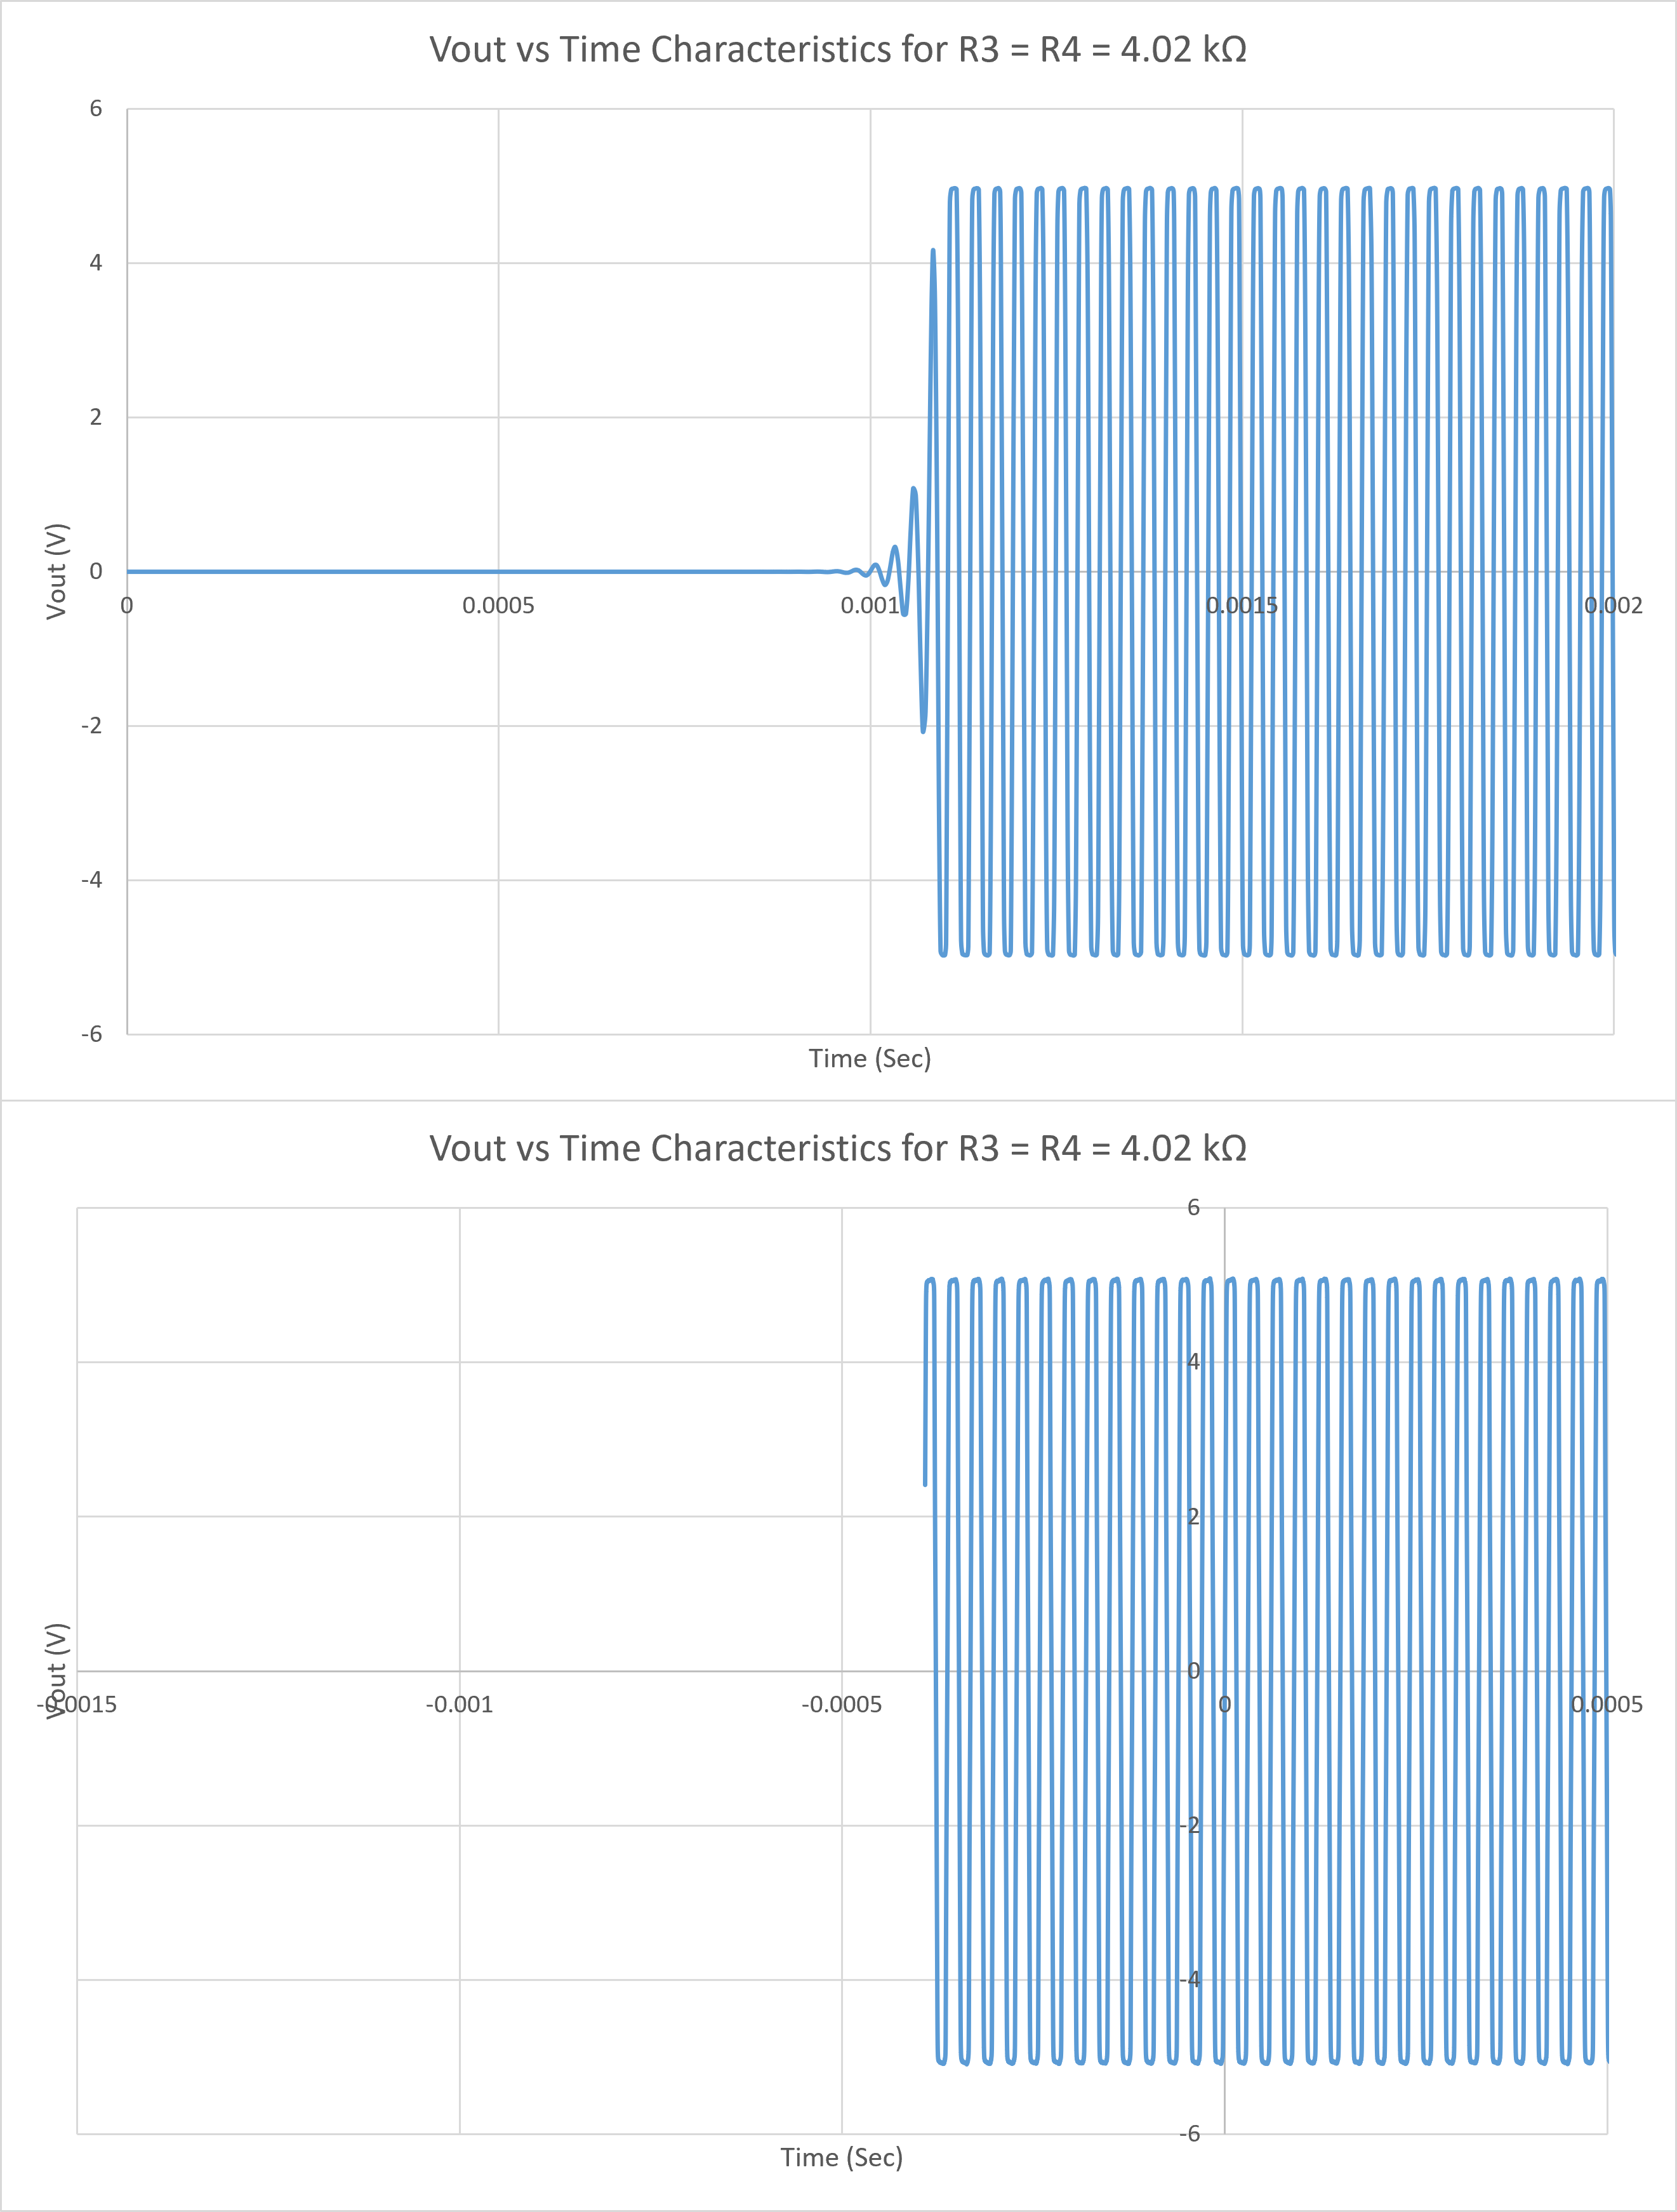
\includegraphics[width=\textwidth]{Q12B}
                \caption{\label{fig:Q12B}Steps 2.6 and 2.10}
            \end{subfigure}
            \caption{\label{fig:Q12} Output voltage $V_o$}
        \end{figure}
        \item The frequencies in Step 2.4 (simulated) and 2.9 (measured) were found to be approximately 17.5 kHz, while the frequencies in Step 2.6 (simulated) and 2.10 (measured) were found be to approximately 33 kHz. This matches the expected results from theory, as the frequency is inversely proportional to the values of R and C ($\omega \propto \frac{1}{RC}$), which was explored in Q9. Therefore, decreasing the value of R to almost half its value (8.25 k$\Omega$ to 4.02 k$\Omega$) nearly doubles the frequency of the oscillations (17.5 kHz to 33 kHz).  
    \end{enumerate}
\end{itemize}
\clearpage
\section*{Appendix}
\begin{figure}[!ht]
    \centering
    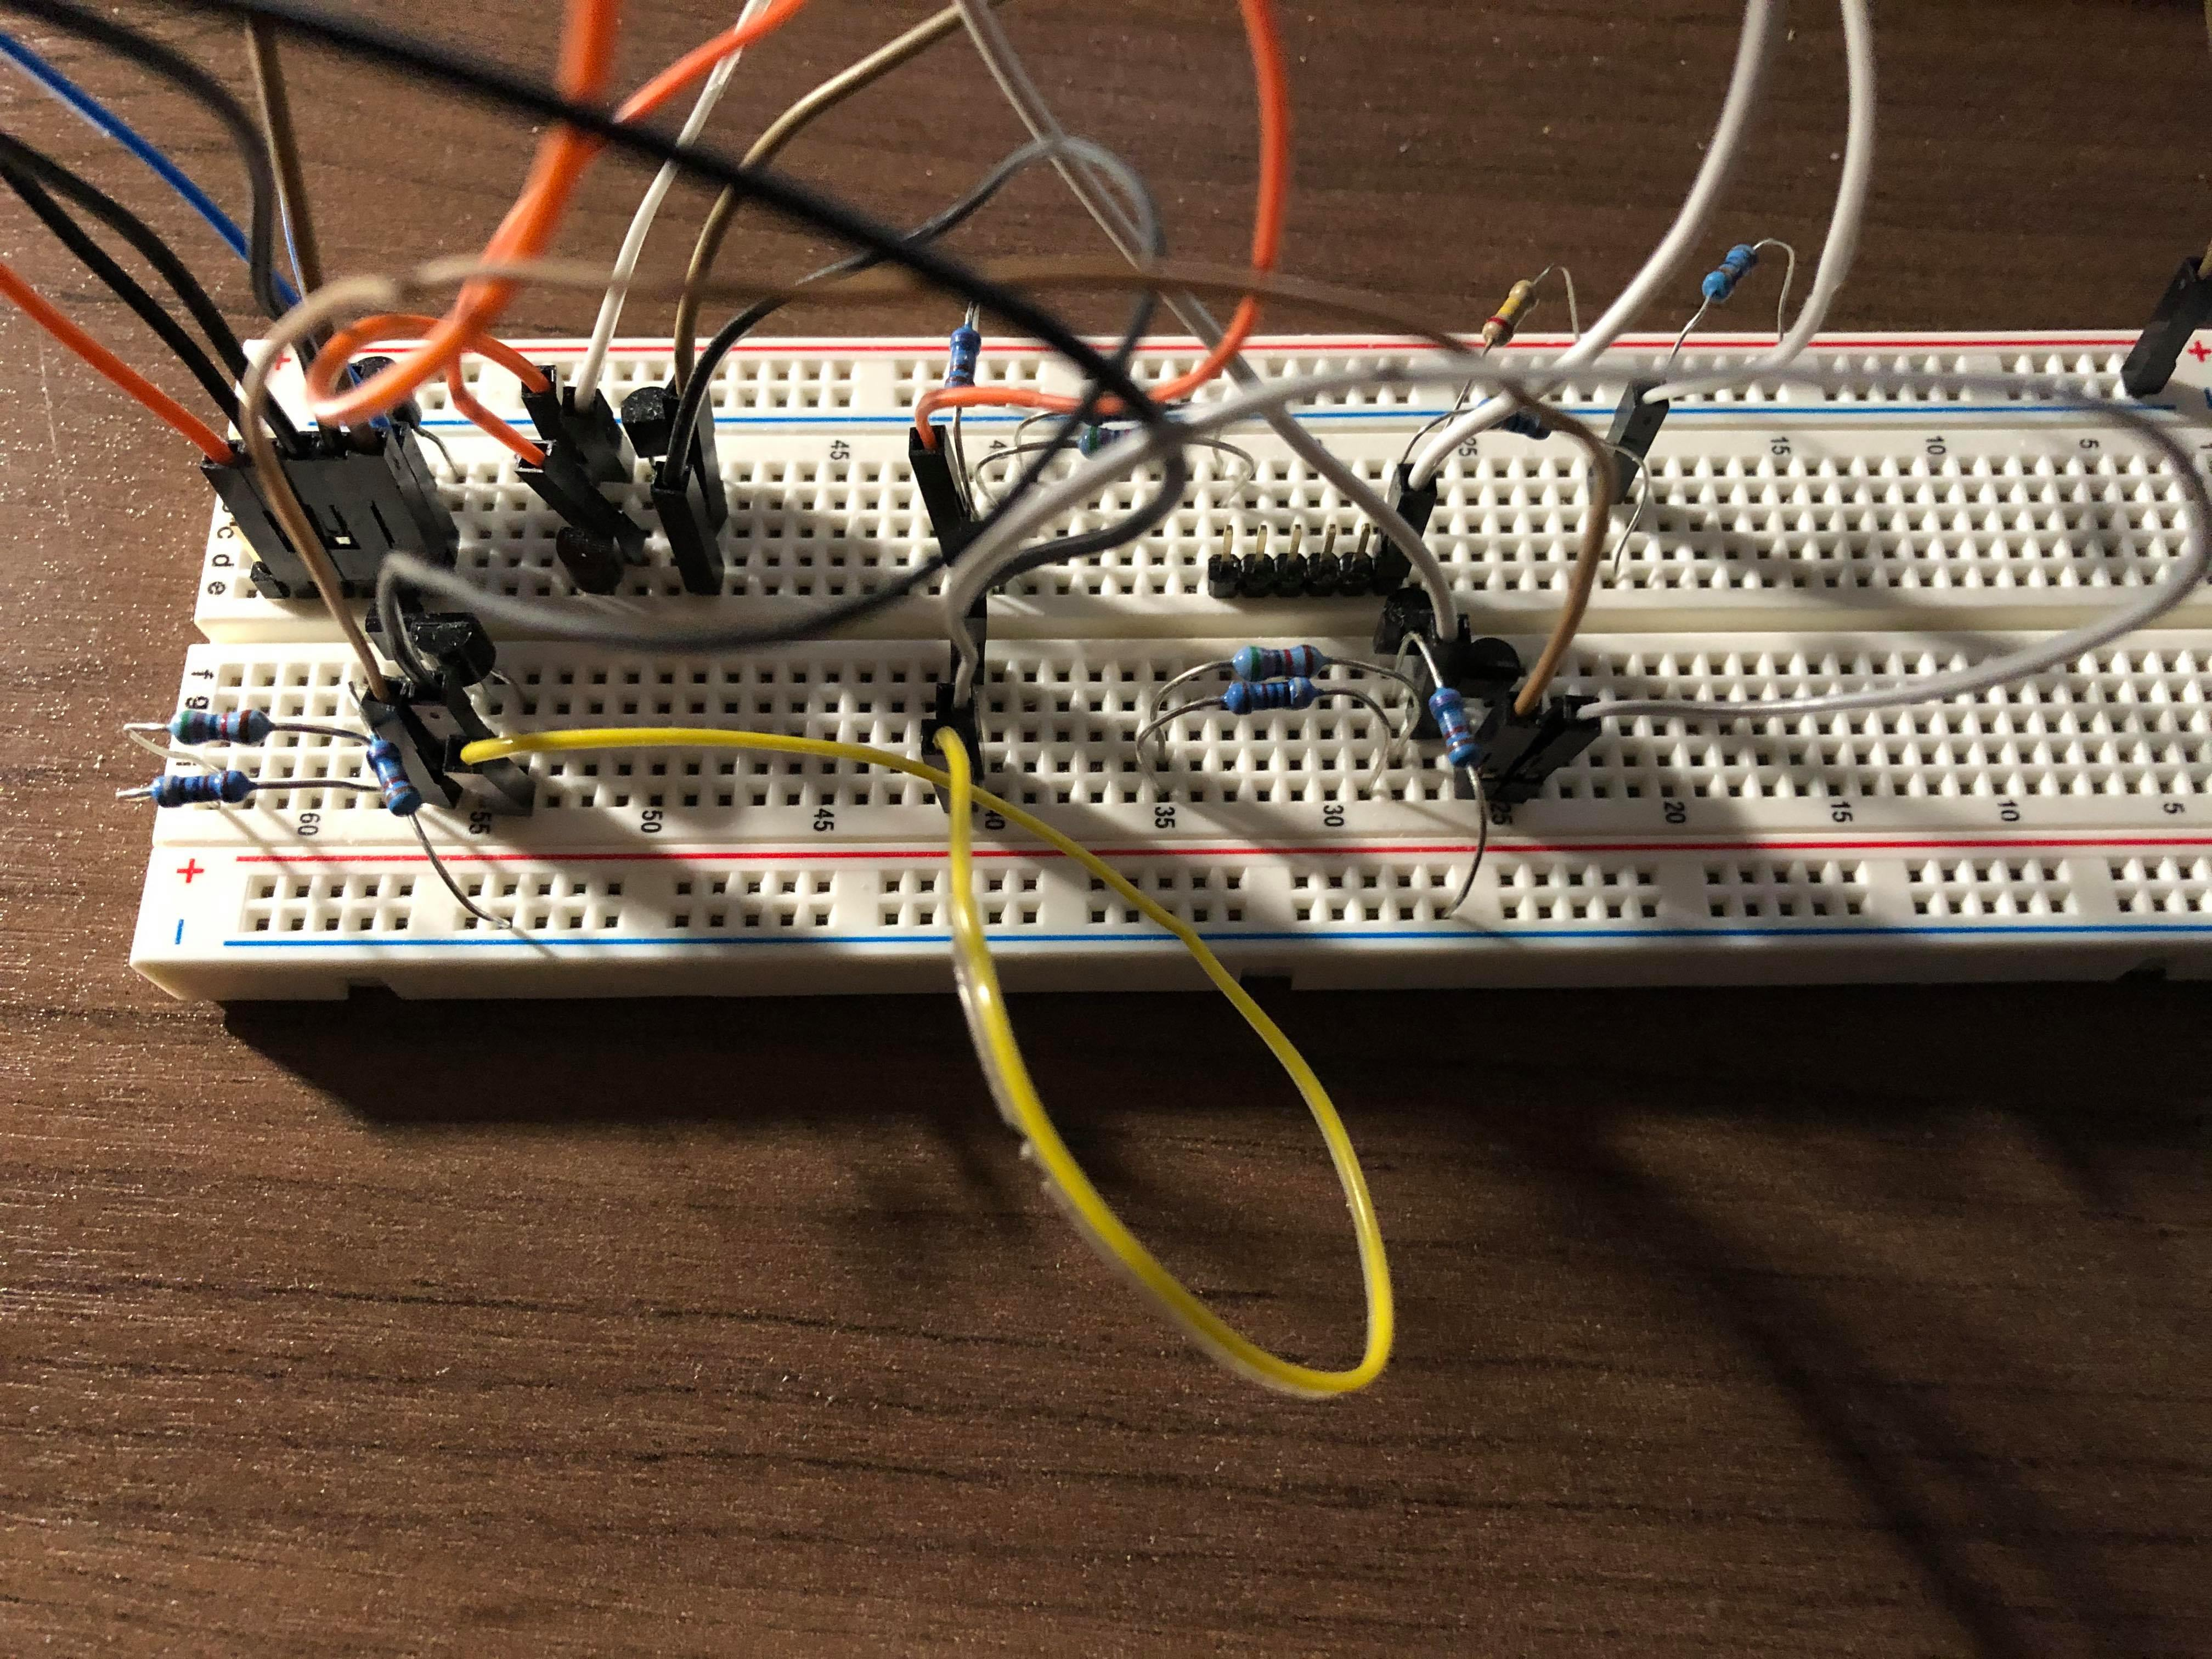
\includegraphics[width=0.7\textwidth]{Part1}
    \caption{\label{fig:P1}Circuit for Part 1}
\end{figure}
\begin{figure}[!ht]
    \centering
    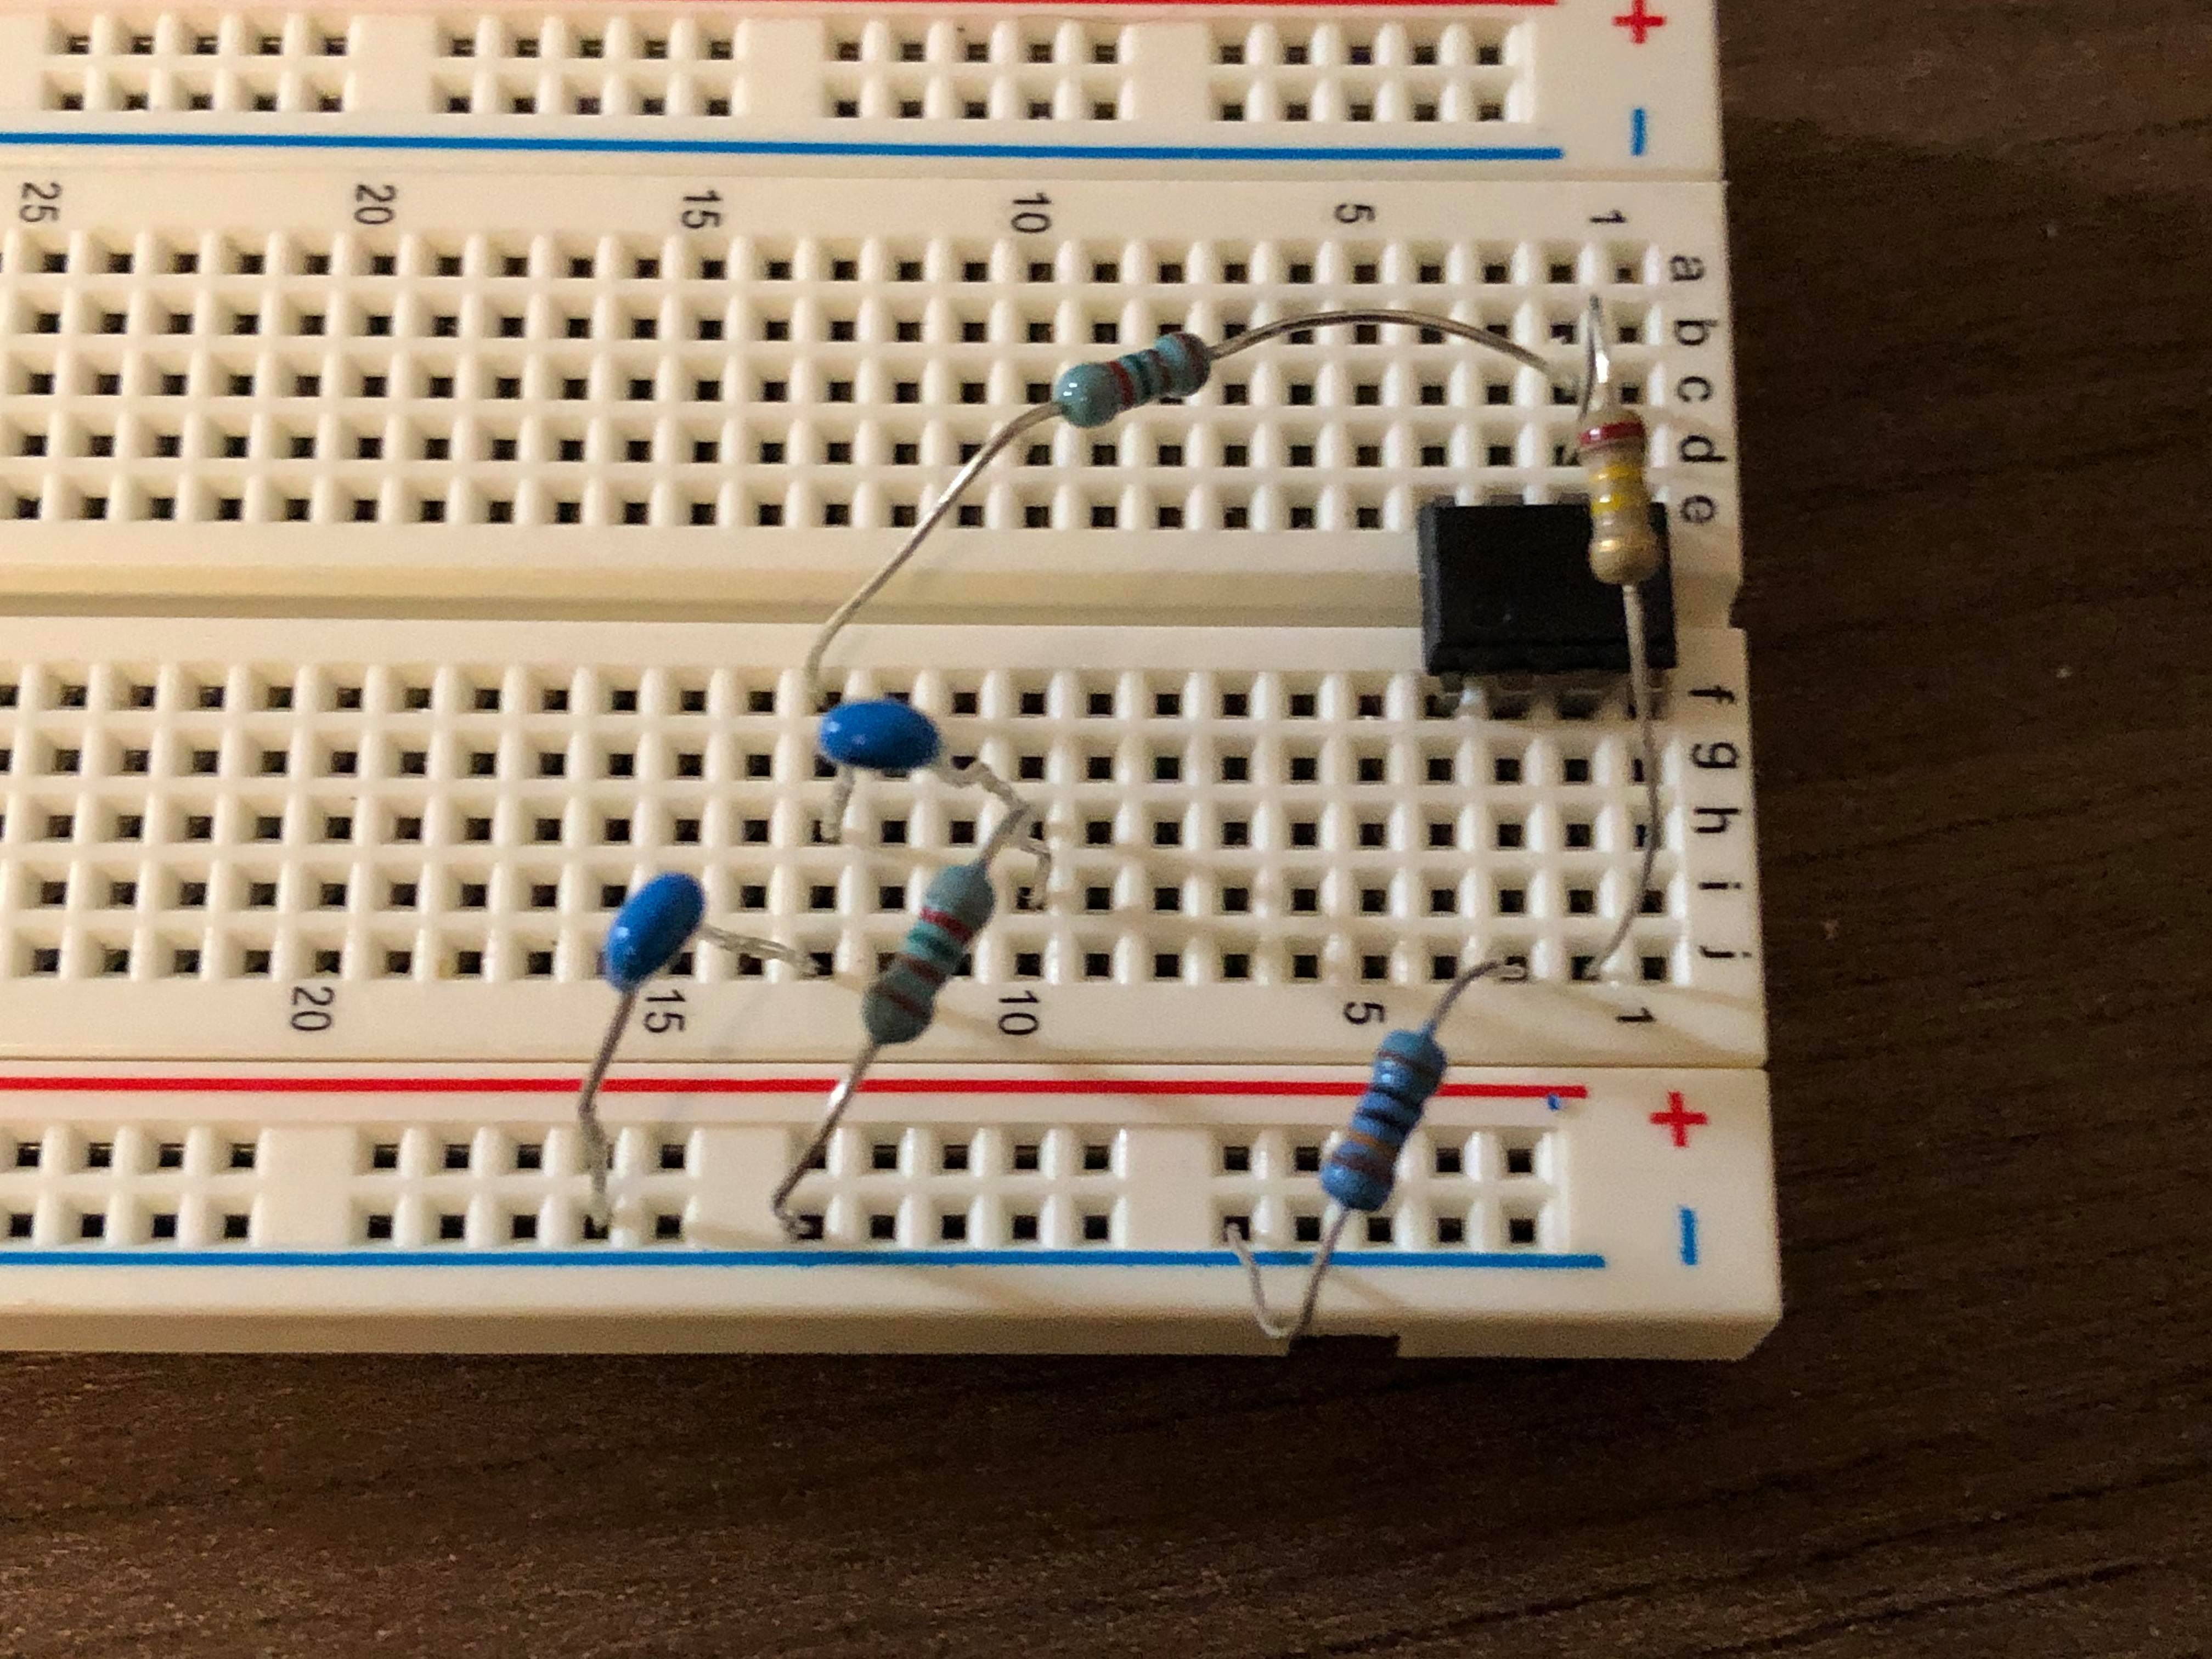
\includegraphics[width=0.7\textwidth]{Part2}
    \caption{\label{fig:P2}Circuit for Part 2}
\end{figure}
\end{document}